\documentclass{ruschidoc}

\usepackage[
	bookmarks,	
	plainpages={false}]{hyperref}

\usepackage[
	style=altlist,
	toc=true,
 	acronym=true]{glossaries}
\usepackage{capt-of}

%%% Water mark 
%\usepackage{draftwatermark}
%\SetWatermarkText{\shortstack{DRAFT}}
%\SetWatermarkScale{0.9}
%\SetWatermarkLightness{0.85}


\makeglossaries
\newacronym{LSB}{LSB}{Least Significant Bit}
\newacronym{MSB}{MSB}{Most Significant Bit}
\newacronym{SoC}{SoC}{System on Chip}
\newacronym{AES}{AES}{Advanced Encryption Standard}
\newacronym{ECB}{ECB}{Electronic Code Book}
\newacronym{FSM}{FSM}{Finite State Machine}
\newacronym{NIST}{NIST}{National Institute of Standards and Technology}


\bibliographystyle{IEEEtran}

%%%%%%%%%%%%%%%%%
% Document variables
%%%%%%%%%%%%%%%%%
\docDate{ \today }
\docID{avs\_aes\_doc}
\docRevision{0.8}
\docStatus{Final}
\docTitle{\mbox{AES 128/192/256 (ECB)}  \mbox{Avalon\rtm-MM Slave}}
\keywords{Avalon, bus, slave, cryptography, AES, ecb, IP core }

\authorName{\mbox{Thomas Ruschival} \\ and opencores.org}
\authorURL{www.opencores.org}
\authorAddress{\mbox{}}
\authorEmail{ruschi@opencores.org}


%%%%%%%%%%%%%%%%%%%%%%%%%%%%%%%%%%%%%%%%%%%%%
% FORMAT: Rev | Chapter |  Description | Date | Reviewer \\
\revisionList{ 
0.1 & all & initial document & 2009/02/01  & T. Ruschival \\
0.2 & all & added interrupt  & 2009/03/25  & T. Ruschival \\
0.3 & all & added generics  & 2009/04/20  & T. Ruschival \\
0.4 & all & cleanup for opencores.org  & 2009/05/20  & T. Ruschival \\
0.5 & all & final release  & 2010/03/07  & T. Ruschival \\
0.6 & 3,6 & fixed memory map, added testbench description  & 2010/04/02  & T. Ruschival \\
0.7 & 3,6 & fixed typos  & 2010/04/03  & T. Ruschival \\
0.8 & 6 & corrected key schedule  & 2011/05/15  & T. Ruschival \\
}
%%%%%%%%%%%%%%%%%%%%%%%%%%%%%%%%%%%%%%%%%%%%%


\begin{document}
\maketitle
\newpage
\tableofcontents
\newpage

\section{Introduction}
\label{sec:intro} The \gls{AES} is a symmetric block cipher operating on fixed block sizes
of 128 Bit and is specified for key sizes of 128, 192 and 256 Bit designed by Joan
Daemen and Vincent Rijmen. The algorithm was standardized by \gls{NIST}. For more
information on the algorithm see \cite{NIST:Fips197}.\\
This component implements an AES encryption decryption data path in \gls{ECB} mode with
either 128,192 or 256 Bit keys.  The key length is determined by generics at compile
time. Also the decryption data path can be disabled by generics if it is not needed
for the application.\\
The component provides an Avalon\rtm\ Memory Mapped (Avalon-MM) slave interface to
connect to an Altera\rtm\ Avalon\rtm\ switch fabric. The Avalon\rtm\ interface is
implemented in a way that it can also be used to connect to a Whishbone master if the
signals are correctly mapped, see \cite{Wiki:AvWb}. For further information about the 
Whishbone bus refer to \cite{OC:WBspec}. \\

\section{Interface}
\label{sec:interface}
The AES core is accessed by the interface described in this section. An Avalon\rtm\
interface was chosen for its simplicity and compatibility with wishbone.  Furthermore
Avalon\rtm\ defines interrupt request signals for slaves which would be separate
signals in a Wishbone implementation.The component can be used both in polling 
mode or can provide an interrupt for signalling. \\
Unfortunately Avalon\rtm\ is an Altera\rtm\ proprietary technology. The actual AES
core however is a self contained entity and can be embedded into other \gls{SoC} bus
interfaces as well or used independently.

\subsection{Configuration Generics}
\label{sec:generics}
The AES core can be configured by generics shown in table \ref{tab:generics},
consequently they are provided by the Avalon\rtm\ interface.

\begin{tabularx}{\textwidth}{|p{33mm}|p{25mm}|X|}
  \hline
  \bf{Generic name} & \bf{type} & \bf{Description}\\ \hline
  \texttt{KEYLENGTH}  \label{gen:keylength}	& NATURAL   & Size of initial user key. Must be 128, 192 or 256 \footnotemark[1] . \\ \hline
  \texttt{DECRYPTION} \label{gen:decryption}  & BOOLEAN  & Enables the instantiation of the decrypt data path if true. \\
\hline
\end{tabularx}
\footnotetext[1]{All other values raise a compilation failure}
\captionof{table}{Component generics}
\label{tab:generics}
Note: \texttt{KEYLENGTH} of 192 fail synthesis with Xilinx ISE \rtm\ because of division by 6 in key schedule that cannot be mapped to shift operations (\texttt{keyexpansion.vhd}).

\subsection{Signals}
\label{sec:signals}
The Avalon\rtm\-MM Slave interface is described in \cite{Altera:Avalon}, the component
implements the signals shown in table \ref{tab:signals}. All signals are synchronous,
sampled at the rising edge of the clock. The type for all signals is \texttt{IEEE1164
    std\_logic} or \texttt{std\_logic\_vector}. For signals wider that 1 Bit the range
is \gls{MSB} \texttt{downto} \gls{LSB}. \\
This components has only output signals driven by registers no input signals are directly combinatorially connected to the
output signals, thus combinational loops are avoided.  All signals are active
high. This component does not support burst transfers.

\begin{tabularx}{\textwidth}{|p{30mm}|p{11mm}|p{11mm}|X|}
  \hline
  \bf{Signal name} & \bf{Width} & \bf{In/Out} & \bf{Description}\\ \hline
  \texttt{clk}  \label{sig:clk}	& 1  &  in  & Avalon\rtm\ bus clock, also used to drive the core. \\ \hline
  \texttt{reset} \label{sig:reset}& 1   &  in  & \emph{Synchronous} reset signal for Avalon\rtm\ bus interface. 
  The core itself is designed without need for reset signals. 
	\\ \hline
  \texttt{writedata} \label{sig:writedata} & 32 &  in  & Input data to write to location designated by \texttt{address}. Bit 31 is most significant Bit. 
	\\  \hline
  \texttt{address}   \label{sig:address}    & 5   &  in & Word offset to the components base address. The memory map of the component for the
  respective offset is described in \ref{sec:memmap}. Only full 32-Bit words can be addressed no byte addressing is implemented.  
	\\  \hline
  \texttt{write}\footnotemark[1] \label{sig:write}  & 1 &  in  & If asserted enable write of data at \texttt{writedata} to location designated by \texttt{address}. 
	\\  \hline
  \texttt{read}\footnotemark[1] \label{sig:read}   & 1 &  in  & If asserted output data at location designated by \texttt{address} to \texttt{readdata}. 
	\\  \hline
  \texttt{readdata} \label{sig:readdata}  & 32  &  out & Data output port for reading data at the location defined by \texttt{address}. Bit 31 is most significant Bit.  
	\\  \hline
 \texttt{waitrequest} \label{sig:waitrequest}  & 1  &  out & Asserted if writedata was not accepted, this is the case if the keyexpansion is
	 not yet complete and a new is written to the \texttt{KEY} address range without previous deassertion of  the \texttt{KEY\_VALID} Bit 
	\\  \hline
  \texttt{irq}\label{sig:irq}   & 1 &  out & If Interrupt behavior is enabled \texttt{IRQ}
  will be asserted when the operation has terminated. For use of interrupt see \ref{sec:irq}  
	\\ \hline
\end{tabularx}
\footnotetext[1]{\texttt{read} and \texttt{write} are mutually exclusive and must not be asserted simultaneously.}
\label{tab:signals}
\captionof{table}{Avalon\rtm\ Bus interface signals}


\section{Memory Map}
\label{sec:memmap}
The AES core Avalon\rtm\ slave has an address space of 31 words accessible through the
offset described by the signal \texttt{address}, see \ref{sig:address}. This address
space is divided into three main sections for the 4-word input data, the 4-word
result of the operation and the user key. The actual length of the user key can vary
between 4, 6 and 8 words depending on the keysize. For control signals and status
information of the component and a control word is provided. The memory mapping is
described in table \ref{tab:memmap}.\\

\begin{tabularx}{\textwidth}{|p{18mm}|p{14mm} |X|}
  \hline
  \bf{Offset} 	  & \bf{Name} & \bf{Description}\\ \hline
  \texttt{0x00-0x07} & \texttt{KEY}  & Initial user key that will be used for encryption and decryption. 
	The most significant word is written to offset \texttt{0x00}. This memory section is \emph{write-only} to the Avalon\rtm\ interface.\\ 
\hline 	 
  \texttt{0x08-0x0B} & \texttt{DATA} & Input data, can be either interpreted as cyphertext for decryption or plain text for encryption. 
	The most significant word shall be written to offset \texttt{0x08}. This memory section is \emph{write-only} to the Avalon\rtm\ interface. \\ 
\hline
  \texttt{0x10-0x13} & \texttt{RESULT} & Result of the operation. The most significant word of the result at offset \texttt{0x10}.  
	This memory section is \emph{read-only} to the Avalon\rtm\ Interface.  \\ 
\hline	 
   \texttt{0x14-0x1E} & --- &  reserved  \\ \hline	 
 \texttt{0x1F} & \texttt{CTRL} & Control and status word of the component can be read and written. Detailed description see \ref{sec:ctrl}\\ 
\hline	
\end{tabularx}
\label{tab:memmap}
\captionof{table}{Memory map of the AES core Avalon\rtm\ slave}

\subsection{Control Register}
\label{sec:ctrl}
The AES Core offers the register \texttt{CTRL} to control the function of the core
and poll its status. The control register can be accessed in read and write mode.
 When writing to the register reserved Bits shall be assigned a value of \texttt{0}.
 Individual Bits have following functionality described in table \ref{tab:ctrlreg}. \\
In case of a Avalon\rtm\ Bus reset this register is set to \texttt{0x00000000} thus
invalidating all previously written keys and resetting the AES core.

\begin{tabularx}{\textwidth}{|p{13mm}|p{18mm} |X|}
  \hline
  \bf{Offset} 	  & \bf{Name} & \bf{Description}\\ \hline
  \texttt{31-8} & --- & reserved \\ \hline 	 
  \texttt{7} 	 &\texttt{KEY\_VALID} &If asserted key data in the \texttt{KEY} memory range is regarded valid and will be expanded to round keys. 
	When deasserted all keys are invalidated and the current operation of the core is aborted. It must be asserted as long as the key shall be 
	used for either encryption or decryption. This bit must be cleared for one clock cycle to load a new key. \\ \hline
  \texttt{6}   & \texttt{IRQ\_ENA}  & Enable use of the interrupt request signal. If asserted the component will set \texttt{IRQ} after 
					completing an operation. If not set the component operates in polling mode only.\\ \hline	 
  \texttt{5-2}   & --- &reserved  \\ \hline	 
  \texttt{1} 	&  \texttt{DEC} \footnotemark[1] &  If asserted memory content of the \texttt{DATA} range is regarded to be valid and will be 
	\emph{decrypted}. This Bit shall only be deasserted externally if a running AES operation is aborted by deasserting \texttt{KEY\_VALID}. 1
	It will be set \texttt{0} by the core to signal completion of the operation.\\ \hline	 
  \texttt{0} 	&  \texttt{ENC} \footnotemark[1] & If asserted memory content of the \texttt{DATA} range is regarded to be valid and will be 
	\emph{encrypted}. This Bit shall only be deasserted externally if a running AES operation is aborted by deasserting \texttt{KEY\_VALID}.
	 It will be set \texttt{0} by the core to signal completion of the operation. \\ \hline	 
\end{tabularx}
\footnotetext[1]{\texttt{ENC} and \texttt{DEC} are mutually exclusive and must not be asserted simultaneously.}
\label{tab:ctrlreg}
\captionof{table}{Bits in the control register}


\section{Protocol Sequence}
\label{sec:usage}
The AES component appears as memory mapped peripheral. All writes are fundamental slave write transfers, see \cite{Altera:Avalon} and take one 
clock cycle of the Avalon\rtm\ bus clock \texttt{clk}. It is not necessary to write all words of a input parameter successively or in one transfer. 
Bursts are not supported.\\
\\
Before any AES operation can be started the initial user key has to be written to
\texttt{KEY} segment of the memory map.After the user key is transferred
to the component the \texttt{KEY\_VALID} Bit must be set to start the key
expansion. This Bit can be set simultaneously with \texttt{DEC} or \texttt{ENC} Bit of
the control register. To invalidate the previous key and use another key the
\texttt{KEY\_VALID} must be deasserted for at least one Avalon\rtm\ bus clock cycle
During this cycle the new key can already be transferred.\\
\\
Once a key is passed and marked valid data blocks can be transferred to the
\texttt{DATA} segment of the memory map. 
The AES operation is started by asserting the \texttt{ENC} Bit for
encryption or \texttt{DEC} Bit for decryption. 
While asserting \texttt{ENC} or \texttt{DEC} the \texttt{KEY\_VALID} Bit must be
kept asserted.\\ 
The \texttt{ENC} or \texttt{DEC} Bit respectively is deasserted by the component
after completing the requested operation.
The result of the operation can be read from the \texttt{RESULT} area of the memory
and is not cleared. It will be overwritten by succeeding operations. 

The underlying AES core uses the \gls{FSM} shown in \ref{fig:aesFSM} for processing of
the data. The signals \texttt{data\_stable} and \texttt{key\_stable} are accessible
over the control status word \texttt{CTRL} \ref{sec:ctrl}. \texttt{key\_ready} is a
signal driven by the key generator when all keys are expanded. The signal
\texttt{round\_index} is the counter for the rounds and the address to select a
round key. \\
\texttt{NO\_ROUNDS} is the total number of rounds the processing takes, a constant
defined by the generic \texttt{KEYLENGTH} \ref{sec:generics}. The AES standard
in\cite{NIST:Fips197} defines 10 rounds for 128 Bit key, 12 rounds for a 192 Bit key
and 14 rounds for a 265 Bit key.\\
Thus depending on the key length the processing of a data block needs at maximum 15
clock cycles from \texttt{data\_stable=1} to completion, if the key is already expanded.

\begin{figure}[!ht]
  \centering
  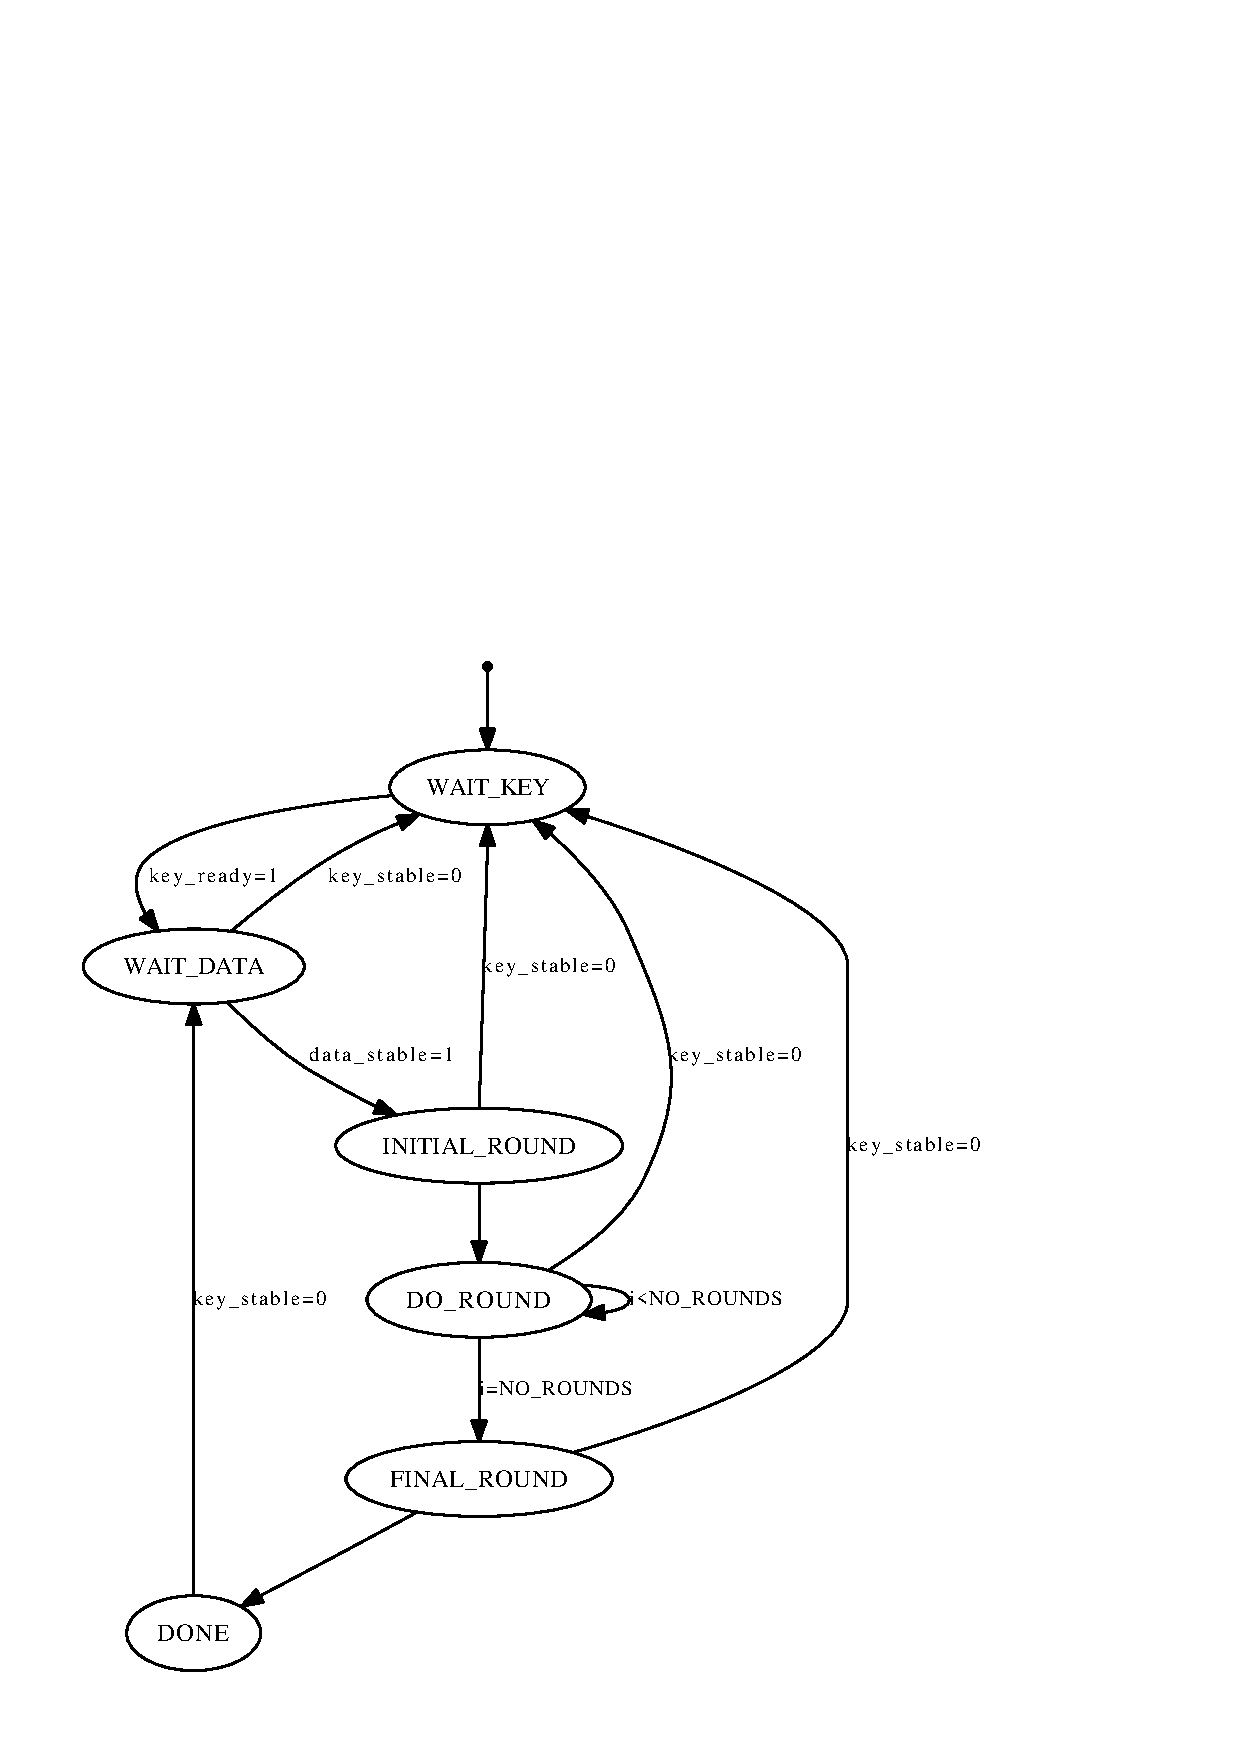
\includegraphics[width=100mm]{encrypt_FSM}
  \caption{Finite State Machine of encryption and decryption process}
  \label{fig:aesFSM}
\end{figure}


\subsection{Interrupt Behavior}
\label{sec:irq}
By setting \texttt{IRQ\_ENA} in the control register \ref{sec:ctrl} the
component is configured to issue interrupt requests.
If \texttt{IRQ\_ENA} is asserted the interrupt request \texttt{IRQ} \ref{sig:irq} will be set when the
computation has completed in addition to clearing the \texttt{ENC} or \texttt{DEC}
Bit.
The \texttt{IRQ} \ref{sig:irq}  signal will remain set until clearing \texttt{IRQ\_ENA}
or a read operation on the \texttt{RESULT} area of the components address range. 

\section{The Inner Core}
\label{sec:core}
The algorithmic core is divided into two separate data paths one for encryption and a
second for decryption operation. The two data paths are independent, however they
share the keyexpansion component which provides decrypt and encrypt keys (which are
the same only in opposite order). Each data path is controlled by its own \gls{FSM}.  If
configured by the generic \texttt{DECRYPTION} \ref{gen:decryption} the decryption
data path is included and some multiplexers are generated for the shared signals,
e.g. \texttt{result} or \texttt{roundkey\_index}.\\
For reference the encryption data path of \texttt{aes\_core.vhd} is given in figure
\ref{fig:aescore}. The decryption data path is left for the reader or any other author
of this document.
\newpage
\begin{figure}[!ht]
  \centering
  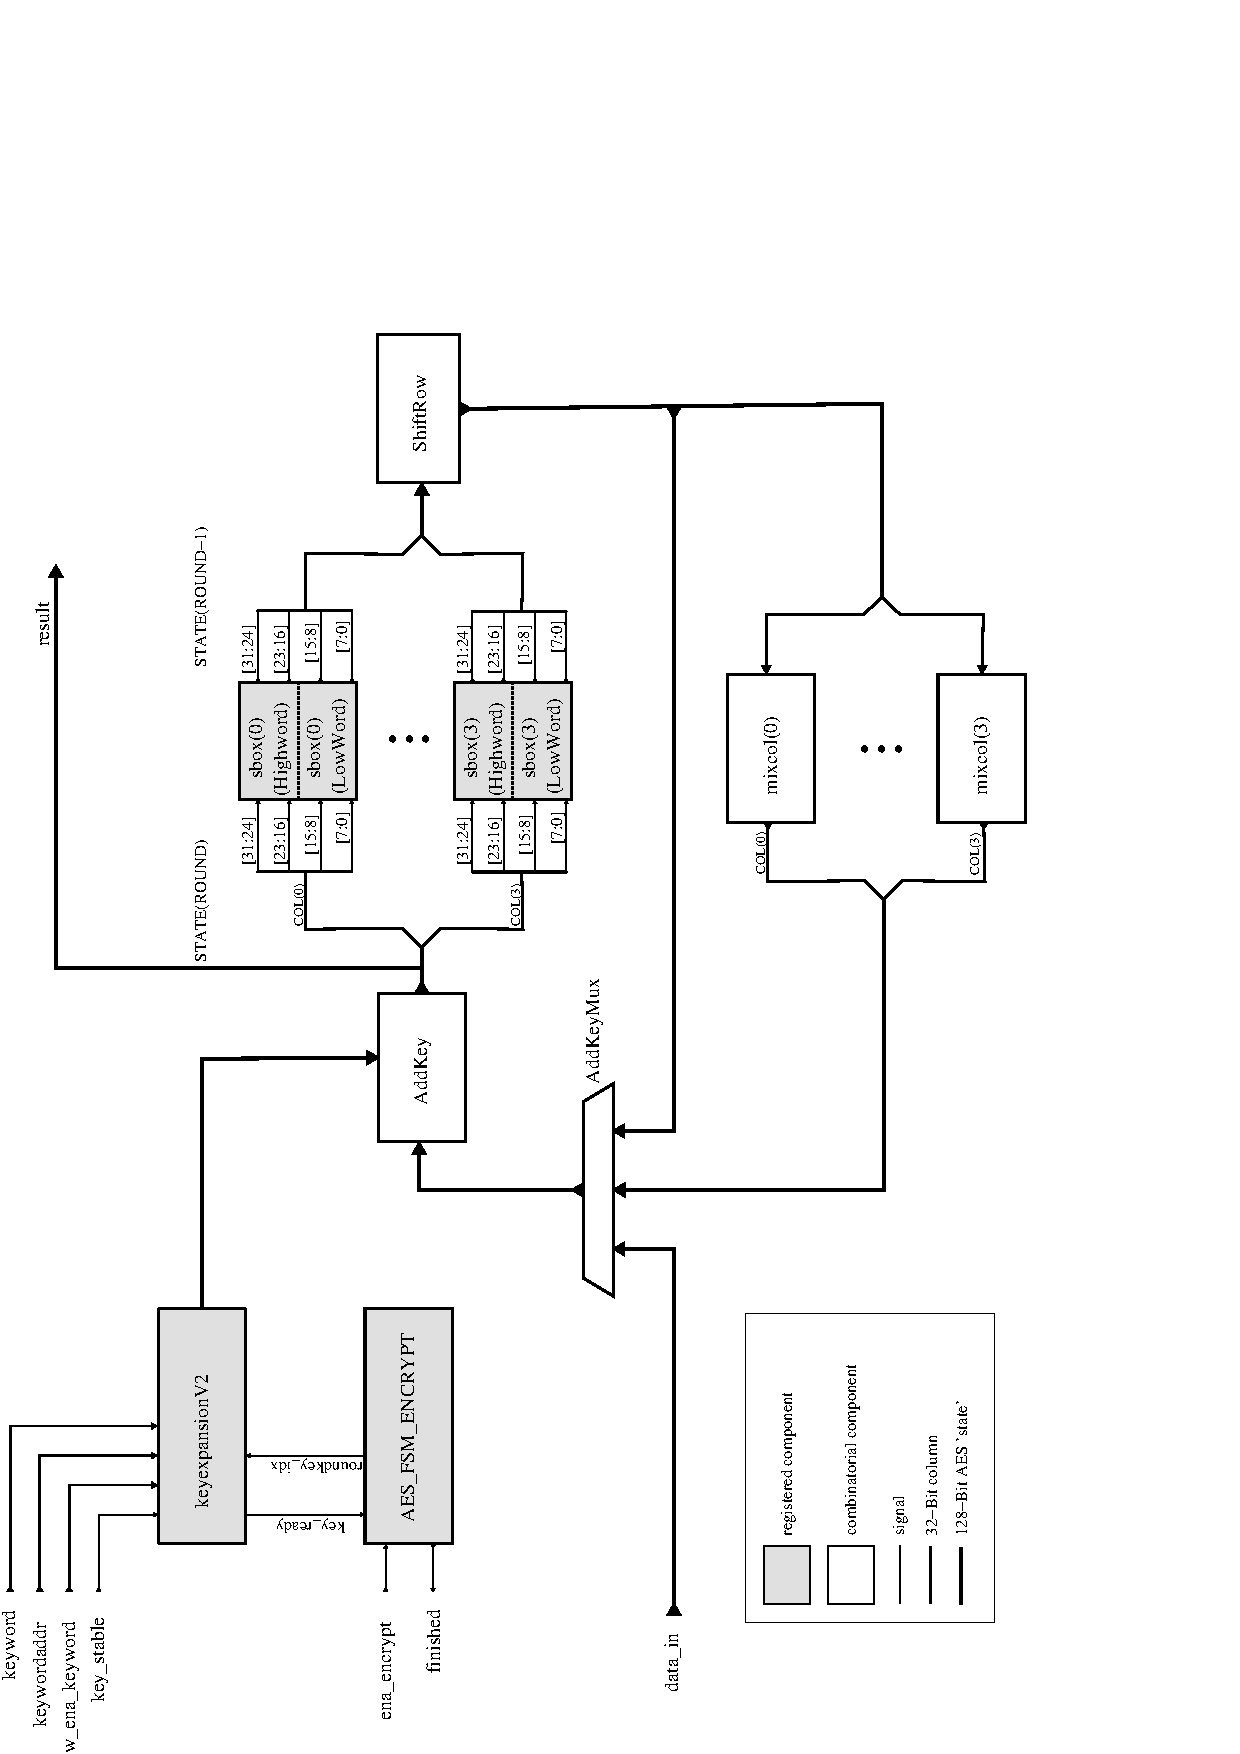
\includegraphics[width=0.9\textwidth]{CoreEncDP}
  \caption{Encrypt data path of the AES core as implemented in aes\_core.vhd}
  \label{fig:aescore}
\end{figure}
\newpage
\section{Throughput Calculation}
\label{sec:throughput}
The Avalon\rtm\ interface communicates a 32-Bit DWORD per clock cycle. Therefore a key is transmitted in 4 to 8 cycles
plus one cycle to activate keyexpansion with the control word \ref{sec:ctrl}. A payload data block or the result consist
always of 4 DWORDs, thus it takes 4 cycles to send data to the core, one cycle to activate the computation with the
control register \ref{sec:ctrl} and 4 cycles to retrieve the data.

The keyexpansion component computes one column of a roundkey in two clock cycles. In
the first cycle the column is substituted throught the s-box, in the second cycle the
shift-operation is executed. AES specifies \cite{NIST:Fips197}, depending on the key length $ N_{roundkeys}=\{10,12,14\} $
roundkeys with 4 columns each. The \gls{FSM} of the keyexpansion module adds o clockcycle for the ``DONE'' state. 
\begin{equation}
  T_{keyexpansion}(N_{roundkeys}) = 2 \cdot 4 \cdot N_{roundkeys} +1 
\label{eqn:keyexp}
\end{equation}
The keyexpansion therefore takes 81, 97 or 115 clockcycles until the encryption or decryption can start. The
roundkeys are stored until invalidated, see \ref{sec:usage} thus this step is is only needed once after power-up until the key changes.

The AES core computes one iteration (round) of the Rijndael-Algorithm each clock cycle, thus a 128 Bit data block is
encrypted or decrypted in 10, 12 or 14 cycles plus an initial round.

The maximum throughput $T_{max}[Bits]$ depends on the maximum operation frequency $f_{max}$ and the key length which
influences the number of rounds $N_{rnd} \epsilon \lbrace 10,12,14 \rbrace $.
\begin{equation}
  T_{max}=\frac{ (1+N_{rnd}) \cdot 128 Bit}{f_{max}} 
\label{eqn:tmax}
\end{equation}

Note: Equation \ref{eqn:tmax} assumes that the roundkeys are already generated and does not include the constant of 4+1+4
Avalon\rtm\ bus cycles for transmission of data, activation and result retrieval.
\newpage
\section{FPGA implementations}
\label{sec:fpga}
The component has only be implemented and tested on an Altera\rtm\ Cyclone-II EP2C35
FPGA. For this setup a Makefile is provided in \texttt{./sys/Altera\_Quartus9.1}.  All
other values in the table are only results of synthesis\footnotemark[0] and are not
verified on actual hardware.

\footnotetext[0]{Synthesized with Altera\rtm\ Quartus-II\rtm\ Web edition Version 9.1 or Xilinx\rtm\ ISE 9.1 Webpack}

The design is kept vendor independent in generic VHDL. 
AES SubByte component is specially designed using M4K block RAM as dual-port ROM. For
non-Altera\rtm\ FPGAs a second VHDL architecture exists also trying to make use of
ROM functions of the target chips however the success varies on RTL compiler
capabilities. Later versions of  Altera\rtm\ Quartus-II\rtm\ show the same results whether M4K blocks are used or the generic version in selected.

\begin{tabularx}{\textwidth}{|p{30mm}|X|p{20mm}|p{30mm}|p{18mm}|}
  \hline
  \bf{Configuration} & \bf{Target FPGA}\footnotemark[1] & \bf{LE / Slices} & \bf{HW RAM} & $\mathbf{f_{max}[Mhz]}$  \\ \hline
	\multirow{4}{30mm}{256 Bit Key, encrypt + decrypt} & \mbox{Xilinx\rtm\ Spartan3A} XC3S1400A-5FG484 &  - / 1609 & 18 RAMB16BWE & 91 \\ \cline{2-5}
	& \mbox{Xilinx\rtm\ Virtex5}   XC5VLX30-3FF324 &  - / 297 & \mbox{18 18k-Blocks}  \mbox{4 36k-Blocks} & 224 \\ \cline{2-5}
	& \mbox{Altera\rtm\ Cyclone-II} EP2C35F484C8 & 1937 / - &  \mbox{39912 Bits} in  \mbox{22 M4K-Blocks} & 65 \\ \cline{2-5}
	& \mbox{Altera\rtm\ StratixII} EP2S30F484C5 & 585 / - &  \mbox{39912 Bits} in  \mbox{22 M4K-Blocks} & 103  \\  
	\hline
%%%%%%
	\multirow{2}{30mm}{128 Bit Key, encrypt + decrypt} & \mbox{Xilinx\rtm\ Spartan3A} XC3S1400A-5FG484 &  - / 1523 & 18 RAMB16BWE & 91 \\ \cline{2-5}
		& \mbox{Altera\rtm\ Cyclone-II} EP2C35F484C8 & 1776 / - &  \mbox{39912 Bits} in  \mbox{22 M4K-Blocks} & 65 \\ 
	\hline
%%%%%%
	\multirow{4}{30mm}{256 Bit Key, encrypt} & \mbox{Xilinx\rtm\ Spartan3A}  XC3S1400A-5FG484 &  - / 680 & 14 RAMB16BWE & 159 \\ \cline{2-5}
	& \mbox{Xilinx\rtm\ Virtex5}   XC5VLX30-3FF324 &  - / 297 & \mbox{10 18k-Blocks}  \mbox{4 36k-Blocks} & 268 \\ \cline{2-5}
	& \mbox{Altera\rtm\ Cyclone-II} EP2C35F484C8 & 969 / - &  \mbox{22528 Bits} in  \mbox{14 M4K} & 97 \\ \cline{2-5}
	& \mbox{Altera\rtm\ StratixII} EP2S30F484C5 & 524 / - &  \mbox{22528 Bits} in \mbox{ 14 M4K} & 145  \\ 
	\hline
%%%%%%
	\multirow{2}{30mm}{128 Bit Key, encrypt} & \mbox{Xilinx\rtm\ Spartan3A}  XC3S1400A-5FG484 &  - / 594 & 14 RAMB16BWE & 159 \\ \cline{2-5}
	& \mbox{Altera\rtm\ Cyclone-II} EP2C35F484C8 & 797 / - & \mbox{22528 Bits} in  \mbox{ 14 M4K} & 95  \\ \cline{2-5} 
	\hline
\end{tabularx}
\footnotetext[1]{This table is not meant to be a benchmark between FPGAs of different vendors, it is only a rough
  estimation for the user of the core. 
	The FPGA families cannot  be compared easily, see also \cite{Xilinx:wp284} and \cite{Altera:01007}for further details. }
\label{tab:ressources}
\captionof{table}{ressource usage on different targets and configuration}

All configurations in table \ref{tab:ressources} use hardware key
expansion. Downloading of software generated roundkeys is not yet supported. The
decryption and encryption data paths share a common keyexpansion block, multiplexing
the address signals is one of the main reasons for regression of the maximum
frequency $f_{max}$ of the configuration compared to encryption only versions. 

\section{Simulation}
\subsection{Testbench}
\label{sec:testbench}
In \texttt{./bench/VHDL/} a ``self-checking testbench'' is provided which runs tests
for a default \texttt{TESTKEYSIZE} is 256 Bit . For different key lengths the
constant \texttt{TESTKEYSIZE} has to be changed appropriately. Expected results for
all test cases and key lengths are included. The expected results were generated by
AES Calculator applet, written by Lawrie Brown from ADFA, Canberra Australia \cite{LaBr05}.  The
testbench consists of a sequence of 5 test cases:
\begin{enumerate}
\item load key1, load data1, encrypt : (basic encryption test)
\item key1, data1, decrypt: (basic decryption test)
\item key1, data1, encrypt: (test if internal state was changed) 
\item key1, data2, encrypt: (encryption test with new data)
\item key2, data2, encrypt: (encryption test with new key) 
\end{enumerate}

\subsection{Simulation}
\label{sec:simulation}
The component library is ``\texttt{avs\_aes\_lib}''. All files are expected to be
compiled into this library as all files depend at least on the package
\texttt{avs\_aes\_lib.avs\_aes\_pkg}. \\
A Makefile for Mentor Graphics\rtm\ Modelsim\rtm\ is given in \texttt{./sim/}. The
default make target \texttt{simaes} will create the library
``\texttt{avs\_aes\_lib}'' and a ``\texttt{work}'' library, compile all files and run
a testbench. \\

\section{Software Driver}
\label{sec:software}
This AES Core Avalon\rtm\ slave was also tested on a NiosII\rtm\ processor.  To use
it in software a simple driver is provided in \texttt{./sw/} among with an example
program of the basic usage. 
The driver consist of the two files \texttt{avs\_aes.c} and \texttt{avs\_aes.h}.
Find more detailed description in the doxygen documentation in \texttt{./doc/sw/html}.

\subsection{Configuration}
To be adapted to different address mappings and key sizes two macros are use in \texttt{avs\_aes.h}:
 \begin{tabularx}{\textwidth}{|p{25mm}|p{25mm} |X|}
  \hline
  \bf{define} 	  &  \bf{default} & \bf{Description}\\ \hline
  \texttt{KEYWORDS} & \texttt{8}  & Key size in 32 Bit words \\ 
\hline 	 
  \texttt{AES\_BASEADDR} & \texttt{0x40000} & Base address at which the AES Core is mapped to the Avalon\rtm\ switch-fabric \\ 
\hline
\end{tabularx}
\label{tab:macros}
\captionof{table}{user changeable macros in header}


\newpage
\section{License and Liability}
\label{sec:license}
The ``AES 128/192/256 (ECB) Avalon\rtm-MM Slave'' component, all its subcomponents
and documentation (like this document you are reading) are published under following
license:\\

Copyright (c) 2009, Thomas Ruschival - All rights reserved.

Redistribution and use in source and binary forms, with or without modification, are
permitted provided that the following conditions are met:
\begin{itemize}
\item Redistributions of source code must retain the above copyright notice, this
  list of conditions and the following disclaimer.
\item Redistributions in binary form must reproduce the above copyright notice, this
  list of conditions and the following disclaimer in the documentation and/or other
  materials provided with the distribution.
\item Neither the name of the organization nor the names of its contributors may be
  used to endorse or promote products derived from this software without specific
  prior written permission.
\end{itemize}
 THIS SOFTWARE IS PROVIDED BY THE COPYRIGHT HOLDERS AND CONTRIBUTORS "AS IS"
 AND ANY EXPRESS OR IMPLIED WARRANTIES, INCLUDING, BUT NOT LIMITED TO, THE
 IMPLIED WARRANTIES OF MERCHANTABILITY AND FITNESS FOR A PARTICULAR PURPOSE
 ARE DISCLAIMED. \\
IN NO EVENT SHALL THE COPYRIGHT HOLDER OR CONTRIBUTORS BE
 LIABLE FOR ANY DIRECT, INDIRECT, INCIDENTAL, SPECIAL, EXEMPLARY,
 OR CONSEQUENTIAL DAMAGES (INCLUDING, BUT NOT LIMITED TO, PROCUREMENT OF
 SUBSTITUTE GOODS OR SERVICES; LOSS OF USE, DATA, OR PROFITS; OR BUSINESS
 INTERRUPTION) HOWEVER CAUSED AND ON ANY THEORY OF LIABILITY, WHETHER IN
 CONTRACT, STRICT LIABILITY, OR TORT (INCLUDING NEGLIGENCE OR OTHERWISE)
 ARISING IN ANY WAY OUT OF THE USE OF THIS SOFTWARE, EVEN IF ADVISED OF
 THE POSSIBILITY OF SUCH DAMAGE\\

 Note: The term ``SOFTWARE'' in the above licence applies in this case not only to
 software as executable code but also to documentation, hardware description or
 compiled netlists for actual target hardware. As Chips generally don't just
 reproduce ``the above copyright notice, this list of conditions and the following
 disclaimer in the documentation and/or other materials provided with the
 distribution'' the data sheet of the product must also contain it.\\

 Altera, Cyclone-II, Stratix-II, Quartus, NIOS and Avalon are registered trademarks of the Altera
 Corporation
 101 Innovation Drive, San Jose CA USA \\
 Xilinx, Spartan3A and Virtex5 are registered trademarks of Xilinx Inc. 2100 Logic Drive, San Jose CA USA \\
 Mentor Graphics and ModelSim are registered trademarks of Mentor Graphics
 Corporation 8005 SW Boeckman Road, Wilsonville OR USA \newpage

\printglossaries 

\bibliography{cited}
\revisionTable

\end{document}
